\subsection{Code Clones}
\begin{frame}{\insertsubsection}
	\begin{mycolumns}
		\todots
	\mynextcolumn
		\todots
	\end{mycolumns}
\end{frame}
% cloning in single-system engineering, levels of clones?
% cloning in the large, considered harmful
% clone-and-own: even more problematic

\subsection{Feature Traceability}
\begin{frame}{\insertsubsection}
	\begin{mycolumns}[widths={40}]
		\mydefinition{Feature Traceability \mysource{\fospl\mypage{54}}}{\mycite{Feature traceability is the ability to trace a feature from the problem space (for example, the feature model) to the solution space (that is, its manifestation in design and code artifacts).}}
		\todo{all terms introduced?}
	\mynextcolumn
		\myexampletight{Feature Traceability with Colored Source Code}{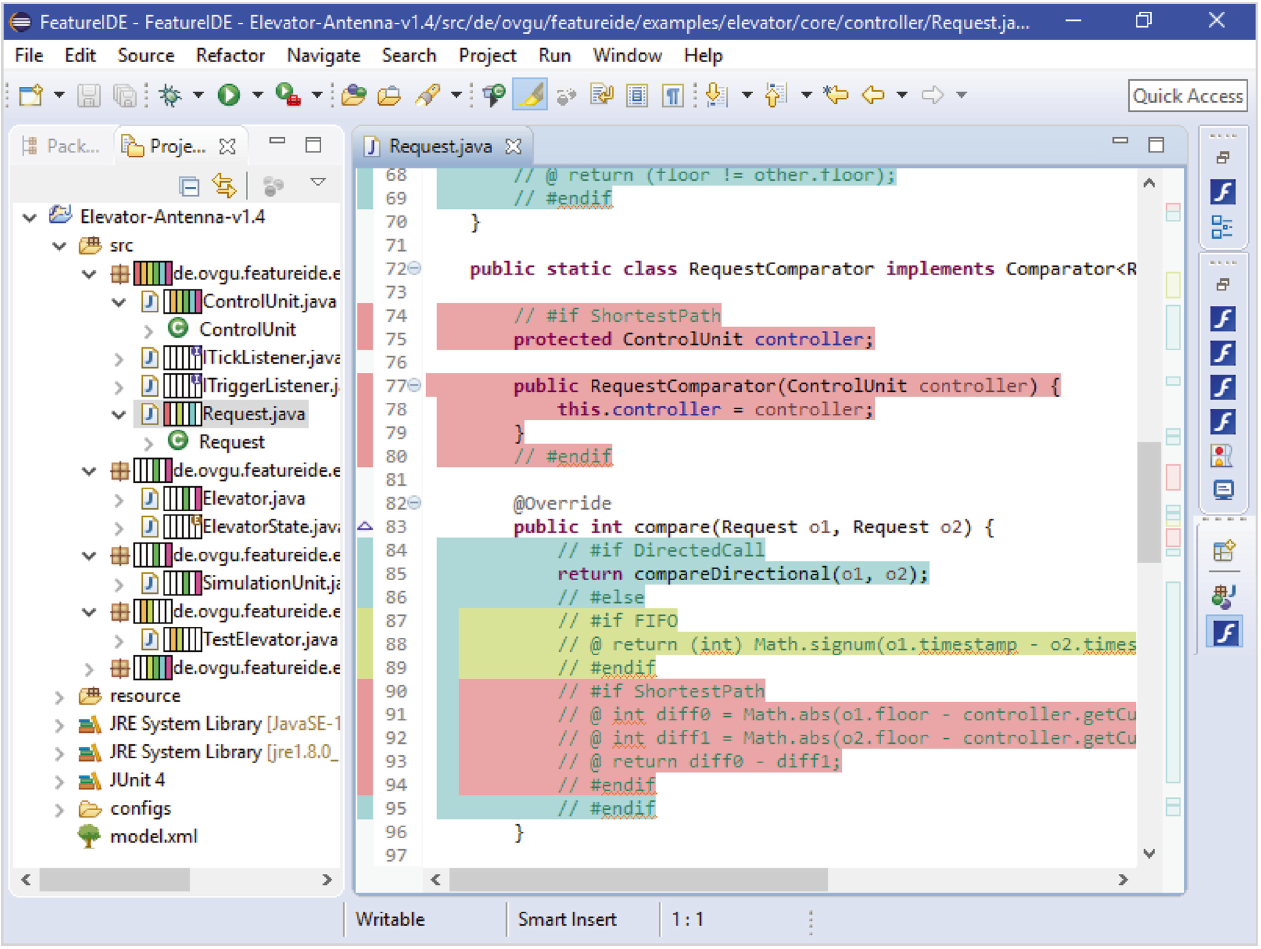
\includegraphics[width=\linewidth]{feature-traceability}}
	\end{mycolumns}
\end{frame}

\subsection{Automated Generation}
\begin{frame}{\insertsubsection}
	\begin{mycolumns}
		\todo{lego pictures}
	\mynextcolumn
		\href{https://pxhere.com/en/photo/920906}{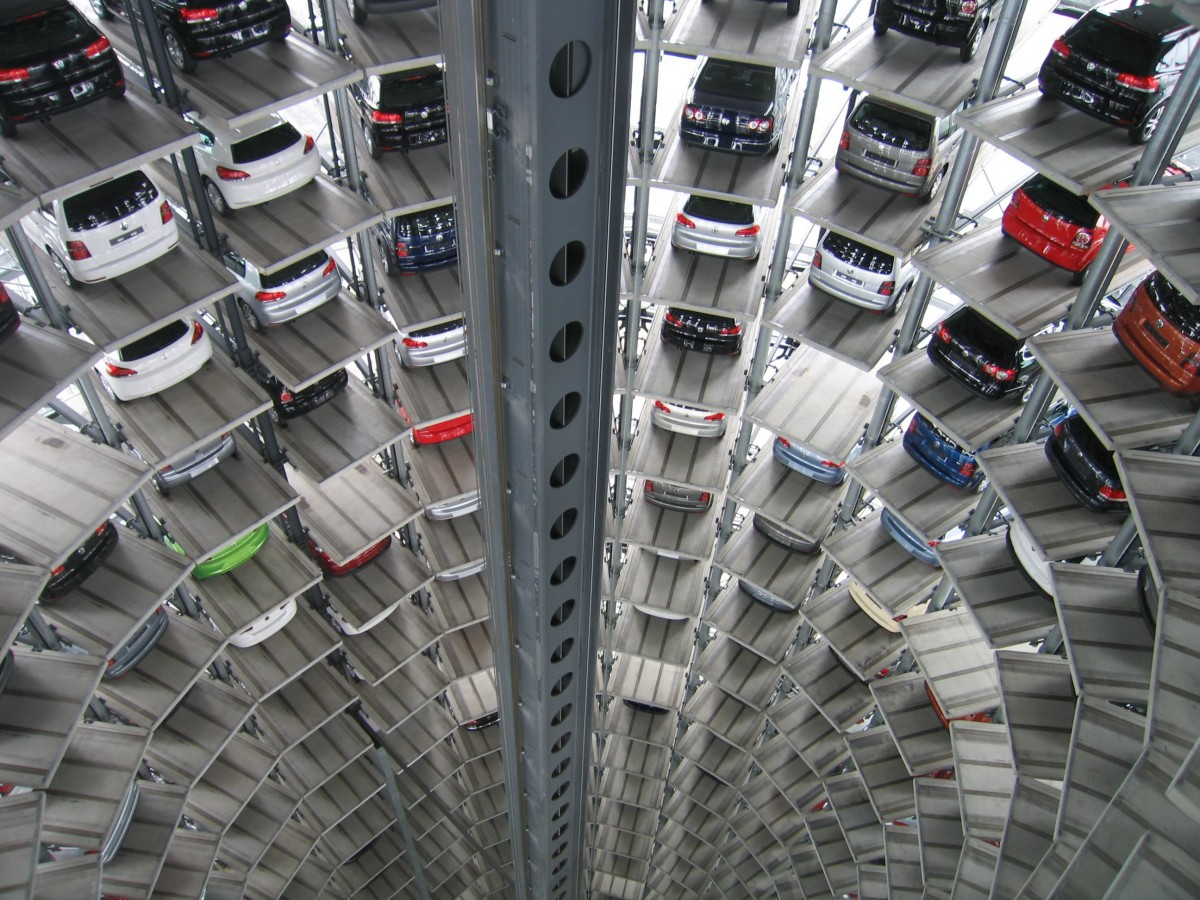
\includegraphics[width=\linewidth]{car-tower}}
	\end{mycolumns}
\end{frame}
% how to automatically generate products given a descriptive selection of features?

\subsection{Combinatorial Explosion}
\begin{frame}{\insertsubsection}
	\begin{mycolumns}[widths={49}]
		\myexampletight{Combinatorial Explosion}{
			\includegraphics[width=\linewidth,page=6]{cit-plots}%
			\small%
			\begin{itemize}
				\item assumption: all combinations of features are valid
				\item 33 features: a unique combination for every human
				\item 320 features: more combinations than atoms in the universe
			\end{itemize}
		}
	\mynextcolumn
		\myexampletight{Industrial Configuration Spaces \mysource{\evaluatingsharpsatsolvers}}{
			\evaluatingsharpsatsolverslink{\includegraphics[width=\linewidth,page=6,trim=50 210 320 440,clip]{2020/2020-VaMoS-Sundermann}}%
			\small%
			\begin{itemize}
				\item in practice: not all combinations of features valid
				\item many industrial product lines too large to specify all valid combinations manually
				\item largest automotive product line has about $1.7 \cdot 10^{1534}$ products
			\end{itemize}
		}
	\end{mycolumns}
\end{frame}
\begin{frame}{\insertsubsection}
	\centering\href{https://github.com/SoftVarE-Group/Slides/blob/main/2021/2021-02-10-VaMoS-SharpSATApplications.pdf}{\includegraphics[height=\textheightwithtitle,page=9,trim=60 15 15 5,clip]{2021/2021-02-10-VaMoS-SharpSATApplications}}
\end{frame}

\subsection{Feature Interactions}
\begin{frame}{\insertsubsection}
	\begin{mycolumns}
		\todots
	\mynextcolumn
		\myexampletight{Invalid Car Configurations}{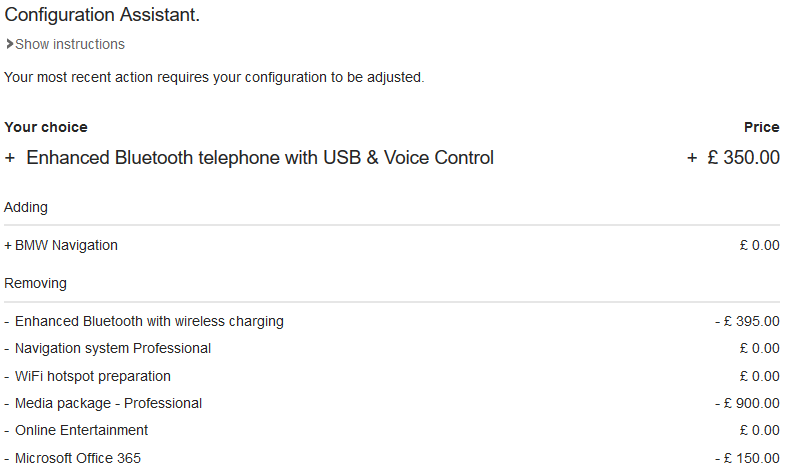
\includegraphics[width=\linewidth]{bmw-series1-confassistant-bluetooth}}
	\end{mycolumns}
\end{frame}
% typically unknown in advance
% quality assurance/correctness necessary

\subsection{Continuing Change and Growth}
\begin{frame}{\insertsubsection}
	\begin{mycolumns}[widths={42}]
		\mydefinition{Lehman's Laws of Software Evolution (excerpt) \mysource{\lehmanslaws}}{
			\begin{itemize}
				\item Continuing Change: systems must be continually adapted to stay satisfactory % E-type systems must be continually adapted else they become progressively less satisfactorv.
				\item Increasing Complexity: complexity increases during evolution unless work is done to maintain or reduce it % As an E-type system evolves its complexity increases unless work is done to maintain or reduce it.
				%\item Self Regulation: %E-type system evolution process is self regulating with distribution of product and process measures close to normal.
				%\item Conservation of Organizational Stability (invariant work rate): %The average effective global activity rate in an evolving E-type system is invariant over product lifetime.
				%\item Conservation of Familiarity: satisfactory evolution excludes excessive growth %As an E-type system evolves all associated with it, developers, sales personnel, users, for example, must maintain mastery of its content and behaviour to achieve satisfactory evolution. Excessive growth diminishes that mastery. Hence the average incremental growth remains invariant as the system evolves.
				\item Continuing Growth: functionality must be continually increased to maintain user satisfaction %The functional content of E-type systems must be continually increased to maintain user satisfaction over their lifetime.
				\item Declining Quality: quality will decline unless rigorously maintained and adapted to operational environment changes %The quality of E-type systems will appear to be declining unless they are rigorously maintained and adapted to operational environment changes.
				%\item Feedback System: %E-type evolution processes constitute multi-level, multi-loop, multi-agent feedback systems and must be treated as such to achieve significant improvement over any reasonable base.
			\end{itemize}
		}
	\mynextcolumn
		\mynote{Essence of the Laws}{
			\begin{itemize}
				\item software that is used will be modified
				\item when modified, its complexity will increase (unless one does actively work against it)
			\end{itemize}
		}
		\myexample{Consequences for Product Lines}{
			\begin{itemize}
				\item number of features and size of implementation increases over time
				\item discussed challenges increase over time
					\begin{itemize}
						\item more code clones
						\item harder to trace features
						\item automated generation more urgent
						\item increasing combinatorial explosion
						\item more feature interactions
					\end{itemize}
			\end{itemize}
		}
	\end{mycolumns}
\end{frame}

\begin{frame}{Evolution of the Linux Kernel}
	\begin{mycolumns}
		\myexample{}{
			\begin{itemize}
				\item about $60,000$ commits per year
				\item in peak weeks: new commit every 5 minutes
				\item in average weeks: every 9 minutes
			\end{itemize}
		}
	\mynextcolumn
		\vspace{-12mm} % TODO Benno: hack. not sure how to improve this.
		\href{https://github.com/erikbern/git-of-theseus}{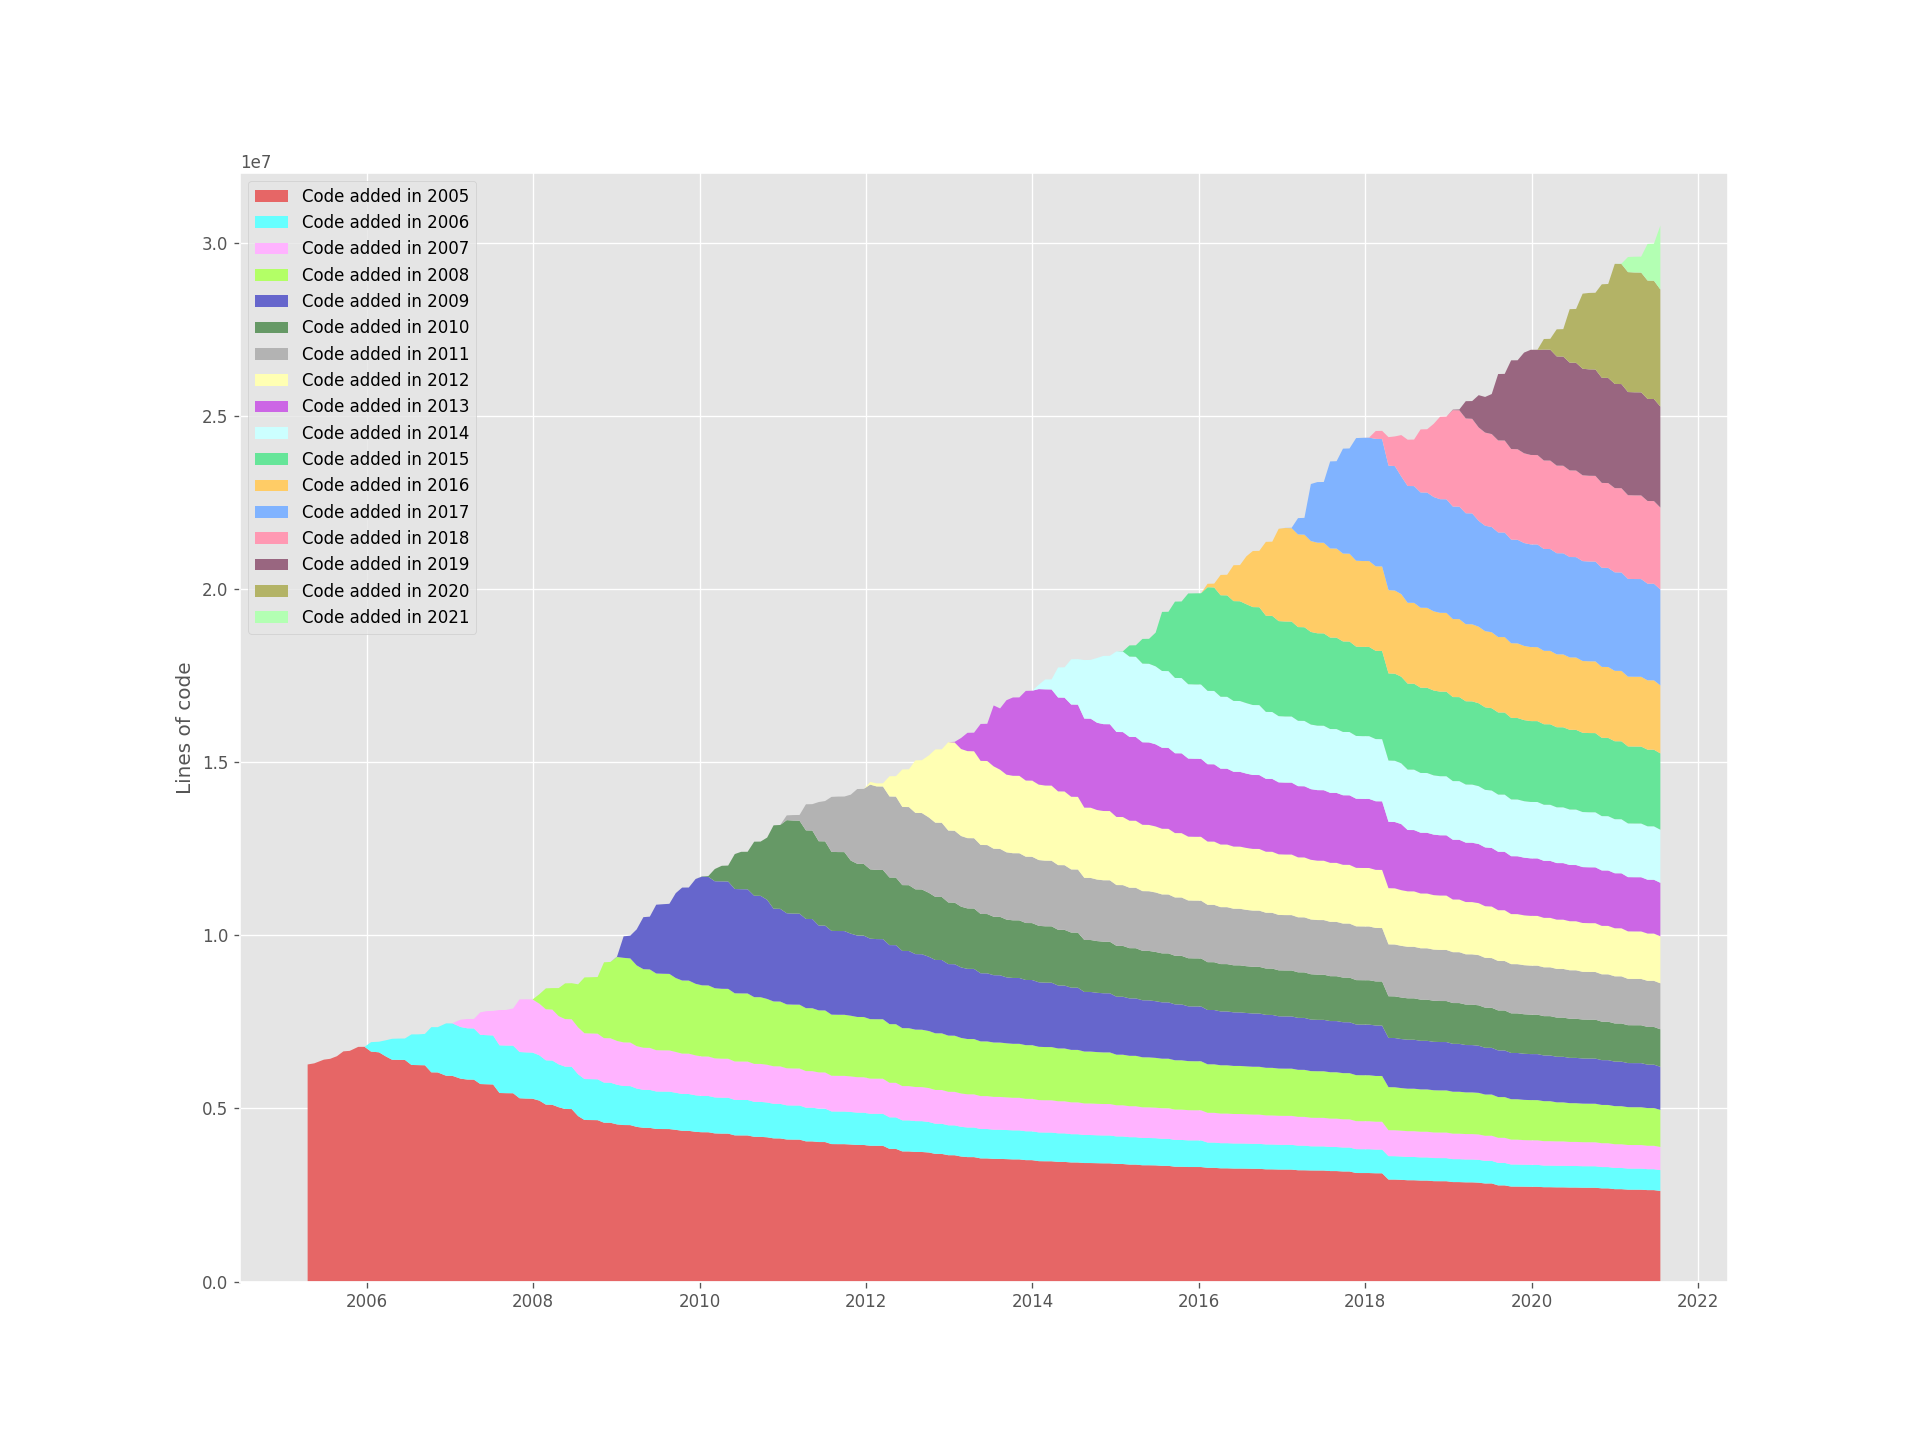
\includegraphics[width=\linewidth,trim=100 70 110 80,clip]{linux-stack-plot}}
	\end{mycolumns}
	\twodimensionalanalysislink{\includegraphics[width=.8\linewidth,page=1,trim=80 420 80 260,clip]{2019/2019-VariVolution-Thuem}}
\end{frame}

\begin{frame}{Evolution of the Linux Kernel}
	\begin{mycolumns}
		\myexampletight{Size of the Code Base}{
			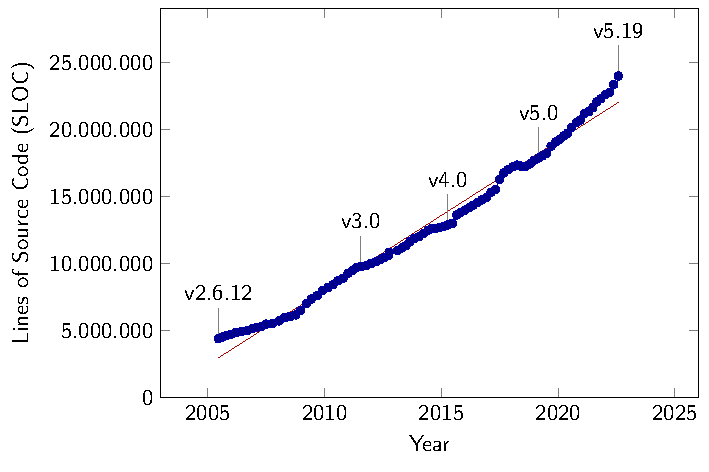
\includegraphics[width=\linewidth,page=1]{linux-plots}%
			\begin{itemize}
				\item from 4 to 24 millions in 17 years
				\item about one million LOC added every year
				\item about 3,000 LOC per day
			\end{itemize}
		}
	\mynextcolumn
		\myexampletight{Number of Features}{
			\includegraphics[width=\linewidth,page=2]{linux-plots}%
			\begin{itemize}
				\item about 800 new features every year
				\item about 15 new features every week
				\item in 2018 four times more features than in 2005
			\end{itemize}
		}
	\end{mycolumns}
\end{frame}

\begin{frame}{Evolution of the Linux Kernel}
	\begin{mycolumns}
		\myexampletight{Number of Products}{
			\includegraphics[width=\linewidth,page=3]{linux-plots}%
			\begin{itemize}
				\item number of products is doubled more than three times a day
				\item the current kernel is likely to have between $10^{6000}$ and $10^{8000}$ products
			\end{itemize}
		}
	\mynextcolumn
		\myexampletight{Time to Count Products}{
			\includegraphics[width=\linewidth,page=4]{linux-plots}%
			\begin{itemize}
				\item most kernel versions before 2015 can be computed within 1 minute
				\item most kernel versions after 2015 cannot be computed within 1 hour
			\end{itemize}
		}
	\end{mycolumns}
\end{frame}

% costs: development, investment, maintenance, logistic, production
% customer needs?

